\documentclass[twoside]{book}

% Packages required by doxygen
\usepackage{fixltx2e}
\usepackage{calc}
\usepackage{doxygen}
\usepackage[export]{adjustbox} % also loads graphicx
\usepackage{graphicx}
\usepackage[utf8]{inputenc}
\usepackage{makeidx}
\usepackage{multicol}
\usepackage{multirow}
\PassOptionsToPackage{warn}{textcomp}
\usepackage{textcomp}
\usepackage[nointegrals]{wasysym}
\usepackage[table]{xcolor}

% Font selection
\usepackage[T1]{fontenc}
\usepackage[scaled=.90]{helvet}
\usepackage{courier}
\usepackage{amssymb}
\usepackage{sectsty}
\renewcommand{\familydefault}{\sfdefault}
\allsectionsfont{%
  \fontseries{bc}\selectfont%
  \color{darkgray}%
}
\renewcommand{\DoxyLabelFont}{%
  \fontseries{bc}\selectfont%
  \color{darkgray}%
}
\newcommand{\+}{\discretionary{\mbox{\scriptsize$\hookleftarrow$}}{}{}}

% Page & text layout
\usepackage{geometry}
\geometry{%
  a4paper,%
  top=2.5cm,%
  bottom=2.5cm,%
  left=2.5cm,%
  right=2.5cm%
}
\tolerance=750
\hfuzz=15pt
\hbadness=750
\setlength{\emergencystretch}{15pt}
\setlength{\parindent}{0cm}
\setlength{\parskip}{3ex plus 2ex minus 2ex}
\makeatletter
\renewcommand{\paragraph}{%
  \@startsection{paragraph}{4}{0ex}{-1.0ex}{1.0ex}{%
    \normalfont\normalsize\bfseries\SS@parafont%
  }%
}
\renewcommand{\subparagraph}{%
  \@startsection{subparagraph}{5}{0ex}{-1.0ex}{1.0ex}{%
    \normalfont\normalsize\bfseries\SS@subparafont%
  }%
}
\makeatother

% Headers & footers
\usepackage{fancyhdr}
\pagestyle{fancyplain}
\fancyhead[LE]{\fancyplain{}{\bfseries\thepage}}
\fancyhead[CE]{\fancyplain{}{}}
\fancyhead[RE]{\fancyplain{}{\bfseries\leftmark}}
\fancyhead[LO]{\fancyplain{}{\bfseries\rightmark}}
\fancyhead[CO]{\fancyplain{}{}}
\fancyhead[RO]{\fancyplain{}{\bfseries\thepage}}
\fancyfoot[LE]{\fancyplain{}{}}
\fancyfoot[CE]{\fancyplain{}{}}
\fancyfoot[RE]{\fancyplain{}{\bfseries\scriptsize Generated by Doxygen }}
\fancyfoot[LO]{\fancyplain{}{\bfseries\scriptsize Generated by Doxygen }}
\fancyfoot[CO]{\fancyplain{}{}}
\fancyfoot[RO]{\fancyplain{}{}}
\renewcommand{\footrulewidth}{0.4pt}
\renewcommand{\chaptermark}[1]{%
  \markboth{#1}{}%
}
\renewcommand{\sectionmark}[1]{%
  \markright{\thesection\ #1}%
}

% Indices & bibliography
\usepackage{natbib}
\usepackage[titles]{tocloft}
\setcounter{tocdepth}{3}
\setcounter{secnumdepth}{5}
\makeindex

% Hyperlinks (required, but should be loaded last)
\usepackage{ifpdf}
\ifpdf
  \usepackage[pdftex,pagebackref=true]{hyperref}
\else
  \usepackage[ps2pdf,pagebackref=true]{hyperref}
\fi
\hypersetup{%
  colorlinks=true,%
  linkcolor=blue,%
  citecolor=blue,%
  unicode%
}

% Custom commands
\newcommand{\clearemptydoublepage}{%
  \newpage{\pagestyle{empty}\cleardoublepage}%
}

\usepackage{caption}
\captionsetup{labelsep=space,justification=centering,font={bf},singlelinecheck=off,skip=4pt,position=top}

%===== C O N T E N T S =====

\begin{document}

% Titlepage & ToC
\hypersetup{pageanchor=false,
             bookmarksnumbered=true,
             pdfencoding=unicode
            }
\pagenumbering{alph}
\begin{titlepage}
\vspace*{7cm}
\begin{center}%
{\Large Hus\+Core \\[1ex]\large 1.\+0 }\\
\vspace*{1cm}
{\large Generated by Doxygen 1.8.14}\\
\end{center}
\end{titlepage}
\clearemptydoublepage
\pagenumbering{roman}
\tableofcontents
\clearemptydoublepage
\pagenumbering{arabic}
\hypersetup{pageanchor=true}

%--- Begin generated contents ---
\chapter{Namespace Index}
\section{Packages}
Here are the packages with brief descriptions (if available)\+:\begin{DoxyCompactList}
\item\contentsline{section}{\mbox{\hyperlink{namespace_hus}{Hus}} }{\pageref{namespace_hus}}{}
\end{DoxyCompactList}

\chapter{Hierarchical Index}
\section{Class Hierarchy}
This inheritance list is sorted roughly, but not completely, alphabetically\+:\begin{DoxyCompactList}
\item \contentsline{section}{Game\+Tree\+Core.\+I\+Child\+Selection\+Service}{\pageref{interface_game_tree_core_1_1_i_child_selection_service}}{}
\begin{DoxyCompactList}
\item \contentsline{section}{Game\+Tree\+Core.\+Child\+Selection\+Service\+Alpha\+A\+M\+AF}{\pageref{class_game_tree_core_1_1_child_selection_service_alpha_a_m_a_f}}{}
\begin{DoxyCompactList}
\item \contentsline{section}{Game\+Tree\+Core.\+Child\+Selection\+Service\+A\+M\+AF}{\pageref{class_game_tree_core_1_1_child_selection_service_a_m_a_f}}{}
\item \contentsline{section}{Game\+Tree\+Core.\+Child\+Selection\+Service\+U\+CT}{\pageref{class_game_tree_core_1_1_child_selection_service_u_c_t}}{}
\end{DoxyCompactList}
\item \contentsline{section}{Game\+Tree\+Core.\+Child\+Selection\+Service\+R\+A\+VE}{\pageref{class_game_tree_core_1_1_child_selection_service_r_a_v_e}}{}
\item \contentsline{section}{Game\+Tree\+Core.\+Child\+Selection\+Service\+Silver\+Alpha\+A\+M\+AF}{\pageref{class_game_tree_core_1_1_child_selection_service_silver_alpha_a_m_a_f}}{}
\end{DoxyCompactList}
\item \contentsline{section}{Game\+Tree\+Core.\+I\+Final\+Child\+Selection\+Service}{\pageref{interface_game_tree_core_1_1_i_final_child_selection_service}}{}
\begin{DoxyCompactList}
\item \contentsline{section}{Game\+Tree\+Core.\+Final\+Child\+Selection\+Service\+M\+AX}{\pageref{class_game_tree_core_1_1_final_child_selection_service_m_a_x}}{}
\item \contentsline{section}{Game\+Tree\+Core.\+Final\+Child\+Selection\+Service\+R\+O\+B\+U\+ST}{\pageref{class_game_tree_core_1_1_final_child_selection_service_r_o_b_u_s_t}}{}
\item \contentsline{section}{Game\+Tree\+Core.\+Final\+Child\+Selection\+Service\+S\+E\+C\+U\+RE}{\pageref{class_game_tree_core_1_1_final_child_selection_service_s_e_c_u_r_e}}{}
\end{DoxyCompactList}
\item \contentsline{section}{Game\+Tree\+Core.\+I\+Game\+Tree\+Node}{\pageref{interface_game_tree_core_1_1_i_game_tree_node}}{}
\end{DoxyCompactList}

\chapter{Class Index}
\section{Class List}
Here are the classes, structs, unions and interfaces with brief descriptions\+:\begin{DoxyCompactList}
\item\contentsline{section}{\mbox{\hyperlink{class_game_tree_core_1_1_child_selection_service_alpha_a_m_a_f}{Game\+Tree\+Core.\+Child\+Selection\+Service\+Alpha\+A\+M\+AF}} \\*A child selection service based on the alpha A\+M\+AF algorithm. }{\pageref{class_game_tree_core_1_1_child_selection_service_alpha_a_m_a_f}}{}
\item\contentsline{section}{\mbox{\hyperlink{class_game_tree_core_1_1_child_selection_service_a_m_a_f}{Game\+Tree\+Core.\+Child\+Selection\+Service\+A\+M\+AF}} \\*A child selection service based on the A\+M\+AF algorithm. This is a special case of the alpha A\+M\+AF version (alpha = 1). }{\pageref{class_game_tree_core_1_1_child_selection_service_a_m_a_f}}{}
\item\contentsline{section}{\mbox{\hyperlink{class_game_tree_core_1_1_child_selection_service_r_a_v_e}{Game\+Tree\+Core.\+Child\+Selection\+Service\+R\+A\+VE}} \\*A child selection service based on the R\+A\+VE algorithm. }{\pageref{class_game_tree_core_1_1_child_selection_service_r_a_v_e}}{}
\item\contentsline{section}{\mbox{\hyperlink{class_game_tree_core_1_1_child_selection_service_silver_alpha_a_m_a_f}{Game\+Tree\+Core.\+Child\+Selection\+Service\+Silver\+Alpha\+A\+M\+AF}} \\*A child selection service based on the alpha A\+M\+AF algorithm from David Silver. }{\pageref{class_game_tree_core_1_1_child_selection_service_silver_alpha_a_m_a_f}}{}
\item\contentsline{section}{\mbox{\hyperlink{class_game_tree_core_1_1_child_selection_service_u_c_t}{Game\+Tree\+Core.\+Child\+Selection\+Service\+U\+CT}} \\*A child selection service based on the U\+CT algorithm. This is a special case of the alpha A\+M\+AF version (alpha = 0). }{\pageref{class_game_tree_core_1_1_child_selection_service_u_c_t}}{}
\item\contentsline{section}{\mbox{\hyperlink{class_game_tree_core_1_1_final_child_selection_service_m_a_x}{Game\+Tree\+Core.\+Final\+Child\+Selection\+Service\+M\+AX}} }{\pageref{class_game_tree_core_1_1_final_child_selection_service_m_a_x}}{}
\item\contentsline{section}{\mbox{\hyperlink{class_game_tree_core_1_1_final_child_selection_service_r_o_b_u_s_t}{Game\+Tree\+Core.\+Final\+Child\+Selection\+Service\+R\+O\+B\+U\+ST}} }{\pageref{class_game_tree_core_1_1_final_child_selection_service_r_o_b_u_s_t}}{}
\item\contentsline{section}{\mbox{\hyperlink{class_game_tree_core_1_1_final_child_selection_service_s_e_c_u_r_e}{Game\+Tree\+Core.\+Final\+Child\+Selection\+Service\+S\+E\+C\+U\+RE}} }{\pageref{class_game_tree_core_1_1_final_child_selection_service_s_e_c_u_r_e}}{}
\item\contentsline{section}{\mbox{\hyperlink{interface_game_tree_core_1_1_i_child_selection_service}{Game\+Tree\+Core.\+I\+Child\+Selection\+Service}} \\*Exposes a method to select a child node from a \mbox{\hyperlink{interface_game_tree_core_1_1_i_game_tree_node}{I\+Game\+Tree\+Node}}. }{\pageref{interface_game_tree_core_1_1_i_child_selection_service}}{}
\item\contentsline{section}{\mbox{\hyperlink{interface_game_tree_core_1_1_i_final_child_selection_service}{Game\+Tree\+Core.\+I\+Final\+Child\+Selection\+Service}} \\*Esposes a method to finally select a child node from a \mbox{\hyperlink{interface_game_tree_core_1_1_i_game_tree_node}{I\+Game\+Tree\+Node}}. }{\pageref{interface_game_tree_core_1_1_i_final_child_selection_service}}{}
\item\contentsline{section}{\mbox{\hyperlink{interface_game_tree_core_1_1_i_game_tree_node}{Game\+Tree\+Core.\+I\+Game\+Tree\+Node}} \\*Represents a node in a game tree. ~\newline
}{\pageref{interface_game_tree_core_1_1_i_game_tree_node}}{}
\end{DoxyCompactList}

\chapter{Namespace Documentation}
\hypertarget{namespace_hus}{}\section{Hus Namespace Reference}
\label{namespace_hus}\index{Hus@{Hus}}
\subsection*{Classes}
\begin{DoxyCompactItemize}
\item 
class \mbox{\hyperlink{class_hus_1_1_hus_game_state}{Hus\+Game\+State}}
\begin{DoxyCompactList}\small\item\em Provides properties and methods for a game state of the H\+US game system. \end{DoxyCompactList}\item 
class \mbox{\hyperlink{class_hus_1_1_hus_move}{Hus\+Move}}
\begin{DoxyCompactList}\small\item\em Provides properties and methods for a move of the H\+US game system. \end{DoxyCompactList}\end{DoxyCompactItemize}

\chapter{Class Documentation}
\hypertarget{class_hus_1_1_hus_game_state}{}\section{Hus.\+Hus\+Game\+State Class Reference}
\label{class_hus_1_1_hus_game_state}\index{Hus.\+Hus\+Game\+State@{Hus.\+Hus\+Game\+State}}


Provides properties and methods for a game state of the H\+US game system.  


Inheritance diagram for Hus.\+Hus\+Game\+State\+:\begin{figure}[H]
\begin{center}
\leavevmode
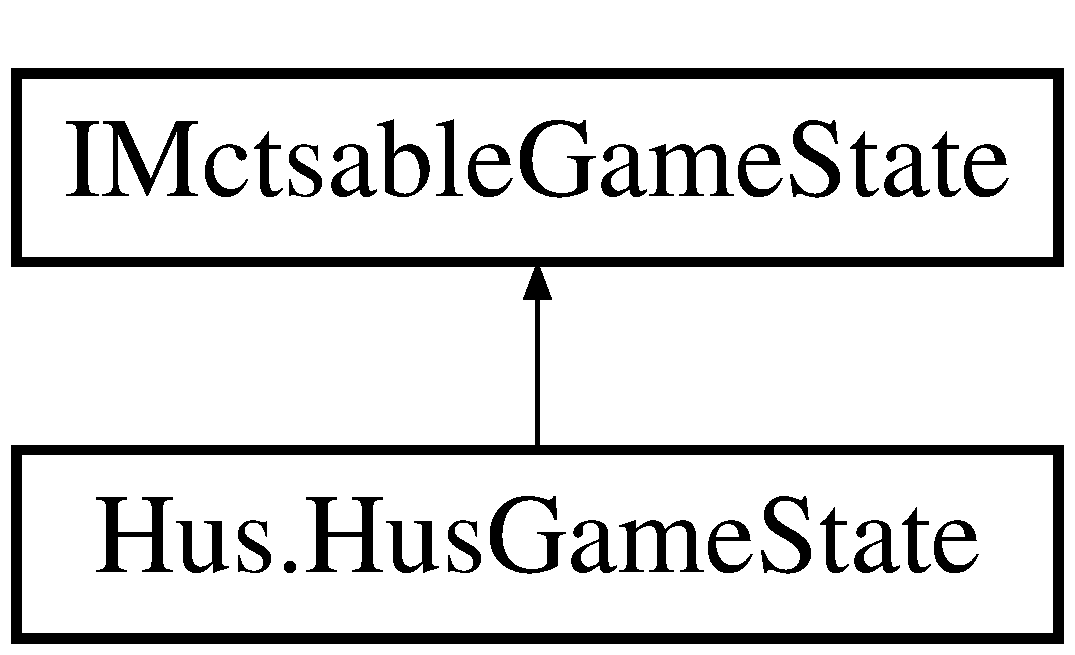
\includegraphics[height=2.000000cm]{class_hus_1_1_hus_game_state}
\end{center}
\end{figure}
\subsection*{Public Member Functions}
\begin{DoxyCompactItemize}
\item 
\mbox{\hyperlink{class_hus_1_1_hus_game_state_ac27c230e200f6c857cd8187c5ffd4cb3}{Hus\+Game\+State}} (int phasing\+Player)
\begin{DoxyCompactList}\small\item\em Creates an inital H\+US game state. \end{DoxyCompactList}\item 
void \mbox{\hyperlink{class_hus_1_1_hus_game_state_a32512f6800dd87707960a5d8ba230abd}{make\+Move}} (I\+Move move)
\begin{DoxyCompactList}\small\item\em Makes the given move. \end{DoxyCompactList}\item 
bool \mbox{\hyperlink{class_hus_1_1_hus_game_state_a9b64d987dbc11c7b6d7035eb9613c633}{is\+Game\+Over}} ()
\begin{DoxyCompactList}\small\item\em Checks, if the game state is a terminal game state. \end{DoxyCompactList}\item 
I\+Mctsable\+Game\+State \mbox{\hyperlink{class_hus_1_1_hus_game_state_ad519755bf09bbc5d4da38aceb3dd27b4}{duplicate}} ()
\begin{DoxyCompactList}\small\item\em Duplicates the game state. \end{DoxyCompactList}\item 
List$<$ I\+Move $>$ \mbox{\hyperlink{class_hus_1_1_hus_game_state_a9fb13d159808e73e86e0c12b4e0dee67}{get\+Possible\+Moves}} ()
\begin{DoxyCompactList}\small\item\em Gets a list of all possible moves. \end{DoxyCompactList}\item 
Game\+Result \mbox{\hyperlink{class_hus_1_1_hus_game_state_aa42355269a96c5df1b46d031548d6e0a}{get\+Result\+Of\+The\+Game}} ()
\begin{DoxyCompactList}\small\item\em Gets the result of a terminal game state. \end{DoxyCompactList}\end{DoxyCompactItemize}
\subsection*{Static Public Attributes}
\begin{DoxyCompactItemize}
\item 
\mbox{\Hypertarget{class_hus_1_1_hus_game_state_ac1917bc0f998d0020b14cdf9a8aee5e1}\label{class_hus_1_1_hus_game_state_ac1917bc0f998d0020b14cdf9a8aee5e1}} 
static int {\bfseries first\+Player} =$>$ \+\_\+\+I\+D\+\_\+\+F\+I\+R\+S\+T\+\_\+\+P\+L\+A\+Y\+ER
\item 
\mbox{\Hypertarget{class_hus_1_1_hus_game_state_a078351292567538d3c41129fe1aa9833}\label{class_hus_1_1_hus_game_state_a078351292567538d3c41129fe1aa9833}} 
static int {\bfseries number\+Of\+Players} =$>$ \+\_\+\+N\+U\+M\+B\+E\+R\+\_\+\+O\+F\+\_\+\+P\+L\+A\+Y\+E\+RS
\item 
\mbox{\Hypertarget{class_hus_1_1_hus_game_state_a81429154fe8cfbe438f7c60f97624291}\label{class_hus_1_1_hus_game_state_a81429154fe8cfbe438f7c60f97624291}} 
static int {\bfseries max\+Pits} =$>$ \+\_\+\+M\+A\+X\+\_\+\+P\+I\+TS
\item 
\mbox{\Hypertarget{class_hus_1_1_hus_game_state_a22c57ee8459880d372162de95a81663a}\label{class_hus_1_1_hus_game_state_a22c57ee8459880d372162de95a81663a}} 
static int {\bfseries second\+Player} =$>$ \+\_\+\+I\+D\+\_\+\+S\+E\+C\+O\+N\+D\+\_\+\+P\+L\+A\+Y\+ER
\end{DoxyCompactItemize}
\subsection*{Properties}
\begin{DoxyCompactItemize}
\item 
\mbox{\Hypertarget{class_hus_1_1_hus_game_state_ac7848176a55c4a95298dd464b83c9f7b}\label{class_hus_1_1_hus_game_state_ac7848176a55c4a95298dd464b83c9f7b}} 
int {\bfseries phasing\+Player}\hspace{0.3cm}{\ttfamily  \mbox{[}get\mbox{]}}
\end{DoxyCompactItemize}


\subsection{Detailed Description}
Provides properties and methods for a game state of the H\+US game system. 



Definition at line 9 of file Hus\+Game\+State.\+cs.



\subsection{Constructor \& Destructor Documentation}
\mbox{\Hypertarget{class_hus_1_1_hus_game_state_ac27c230e200f6c857cd8187c5ffd4cb3}\label{class_hus_1_1_hus_game_state_ac27c230e200f6c857cd8187c5ffd4cb3}} 
\index{Hus\+::\+Hus\+Game\+State@{Hus\+::\+Hus\+Game\+State}!Hus\+Game\+State@{Hus\+Game\+State}}
\index{Hus\+Game\+State@{Hus\+Game\+State}!Hus\+::\+Hus\+Game\+State@{Hus\+::\+Hus\+Game\+State}}
\subsubsection{\texorpdfstring{Hus\+Game\+State()}{HusGameState()}}
{\footnotesize\ttfamily Hus.\+Hus\+Game\+State.\+Hus\+Game\+State (\begin{DoxyParamCaption}\item[{int}]{phasing\+Player }\end{DoxyParamCaption})}



Creates an inital H\+US game state. 


\begin{DoxyExceptions}{Exceptions}
{\em Argument\+Exception} & Is thrown, if the given player is none of the \mbox{\hyperlink{namespace_hus}{Hus}} game.\\
\hline
\end{DoxyExceptions}


Definition at line 36 of file Hus\+Game\+State.\+cs.



\subsection{Member Function Documentation}
\mbox{\Hypertarget{class_hus_1_1_hus_game_state_ad519755bf09bbc5d4da38aceb3dd27b4}\label{class_hus_1_1_hus_game_state_ad519755bf09bbc5d4da38aceb3dd27b4}} 
\index{Hus\+::\+Hus\+Game\+State@{Hus\+::\+Hus\+Game\+State}!duplicate@{duplicate}}
\index{duplicate@{duplicate}!Hus\+::\+Hus\+Game\+State@{Hus\+::\+Hus\+Game\+State}}
\subsubsection{\texorpdfstring{duplicate()}{duplicate()}}
{\footnotesize\ttfamily I\+Mctsable\+Game\+State Hus.\+Hus\+Game\+State.\+duplicate (\begin{DoxyParamCaption}{ }\end{DoxyParamCaption})}



Duplicates the game state. 



Definition at line 138 of file Hus\+Game\+State.\+cs.

\mbox{\Hypertarget{class_hus_1_1_hus_game_state_a9fb13d159808e73e86e0c12b4e0dee67}\label{class_hus_1_1_hus_game_state_a9fb13d159808e73e86e0c12b4e0dee67}} 
\index{Hus\+::\+Hus\+Game\+State@{Hus\+::\+Hus\+Game\+State}!get\+Possible\+Moves@{get\+Possible\+Moves}}
\index{get\+Possible\+Moves@{get\+Possible\+Moves}!Hus\+::\+Hus\+Game\+State@{Hus\+::\+Hus\+Game\+State}}
\subsubsection{\texorpdfstring{get\+Possible\+Moves()}{getPossibleMoves()}}
{\footnotesize\ttfamily List$<$I\+Move$>$ Hus.\+Hus\+Game\+State.\+get\+Possible\+Moves (\begin{DoxyParamCaption}{ }\end{DoxyParamCaption})}



Gets a list of all possible moves. 



Definition at line 145 of file Hus\+Game\+State.\+cs.

\mbox{\Hypertarget{class_hus_1_1_hus_game_state_aa42355269a96c5df1b46d031548d6e0a}\label{class_hus_1_1_hus_game_state_aa42355269a96c5df1b46d031548d6e0a}} 
\index{Hus\+::\+Hus\+Game\+State@{Hus\+::\+Hus\+Game\+State}!get\+Result\+Of\+The\+Game@{get\+Result\+Of\+The\+Game}}
\index{get\+Result\+Of\+The\+Game@{get\+Result\+Of\+The\+Game}!Hus\+::\+Hus\+Game\+State@{Hus\+::\+Hus\+Game\+State}}
\subsubsection{\texorpdfstring{get\+Result\+Of\+The\+Game()}{getResultOfTheGame()}}
{\footnotesize\ttfamily Game\+Result Hus.\+Hus\+Game\+State.\+get\+Result\+Of\+The\+Game (\begin{DoxyParamCaption}{ }\end{DoxyParamCaption})}



Gets the result of a terminal game state. 


\begin{DoxyExceptions}{Exceptions}
{\em Invalid\+Operation\+Exception} & Is thrown, if the game state is not a terminal game state.\\
\hline
\end{DoxyExceptions}


Definition at line 164 of file Hus\+Game\+State.\+cs.

\mbox{\Hypertarget{class_hus_1_1_hus_game_state_a9b64d987dbc11c7b6d7035eb9613c633}\label{class_hus_1_1_hus_game_state_a9b64d987dbc11c7b6d7035eb9613c633}} 
\index{Hus\+::\+Hus\+Game\+State@{Hus\+::\+Hus\+Game\+State}!is\+Game\+Over@{is\+Game\+Over}}
\index{is\+Game\+Over@{is\+Game\+Over}!Hus\+::\+Hus\+Game\+State@{Hus\+::\+Hus\+Game\+State}}
\subsubsection{\texorpdfstring{is\+Game\+Over()}{isGameOver()}}
{\footnotesize\ttfamily bool Hus.\+Hus\+Game\+State.\+is\+Game\+Over (\begin{DoxyParamCaption}{ }\end{DoxyParamCaption})}



Checks, if the game state is a terminal game state. 



Definition at line 98 of file Hus\+Game\+State.\+cs.

\mbox{\Hypertarget{class_hus_1_1_hus_game_state_a32512f6800dd87707960a5d8ba230abd}\label{class_hus_1_1_hus_game_state_a32512f6800dd87707960a5d8ba230abd}} 
\index{Hus\+::\+Hus\+Game\+State@{Hus\+::\+Hus\+Game\+State}!make\+Move@{make\+Move}}
\index{make\+Move@{make\+Move}!Hus\+::\+Hus\+Game\+State@{Hus\+::\+Hus\+Game\+State}}
\subsubsection{\texorpdfstring{make\+Move()}{makeMove()}}
{\footnotesize\ttfamily void Hus.\+Hus\+Game\+State.\+make\+Move (\begin{DoxyParamCaption}\item[{I\+Move}]{move }\end{DoxyParamCaption})}



Makes the given move. 


\begin{DoxyExceptions}{Exceptions}
{\em Argument\+Null\+Exception} & Is thrown, if the given move is null.\\
\hline
{\em Argument\+Exception} & Is thrown, if the given move in invalid, because the pit does not contain enough gems.\\
\hline
{\em Invalid\+Cast\+Exception} & Is thrown, if the given move is not a \mbox{\hyperlink{namespace_hus}{Hus}} move.\\
\hline
\end{DoxyExceptions}


Definition at line 56 of file Hus\+Game\+State.\+cs.


\hypertarget{class_hus_1_1_hus_move}{}\section{Hus.\+Hus\+Move Class Reference}
\label{class_hus_1_1_hus_move}\index{Hus.\+Hus\+Move@{Hus.\+Hus\+Move}}


Provides properties and methods for a move of the H\+US game system.  


Inheritance diagram for Hus.\+Hus\+Move\+:\begin{figure}[H]
\begin{center}
\leavevmode
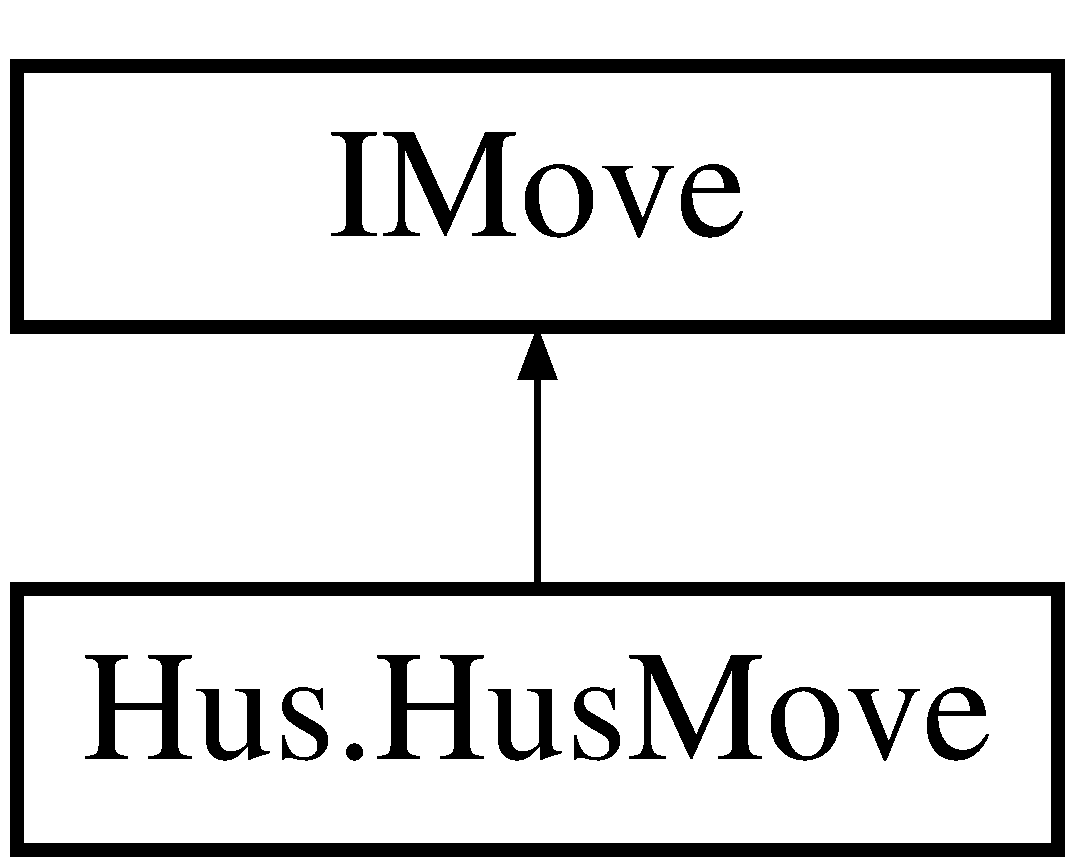
\includegraphics[height=2.000000cm]{class_hus_1_1_hus_move}
\end{center}
\end{figure}
\subsection*{Public Member Functions}
\begin{DoxyCompactItemize}
\item 
\mbox{\hyperlink{class_hus_1_1_hus_move_ad4b8bf3e479f52ac7eb4013a2fd8aba3}{Hus\+Move}} (int player\+Who\+Does\+The\+Move, int next\+Player, int pit)
\begin{DoxyCompactList}\small\item\em Creates a move of the H\+US game system. \end{DoxyCompactList}\item 
bool \mbox{\hyperlink{class_hus_1_1_hus_move_abb8febf6f2c28b760d3c652f05322eb0}{is\+Equal\+To}} (I\+Move move)
\begin{DoxyCompactList}\small\item\em Checks, if the two moves are equal. \end{DoxyCompactList}\end{DoxyCompactItemize}
\subsection*{Properties}
\begin{DoxyCompactItemize}
\item 
\mbox{\Hypertarget{class_hus_1_1_hus_move_a935e6906c622a72f35f59b2d6f5dfaac}\label{class_hus_1_1_hus_move_a935e6906c622a72f35f59b2d6f5dfaac}} 
int {\bfseries next\+Player}\hspace{0.3cm}{\ttfamily  \mbox{[}get\mbox{]}}
\item 
\mbox{\Hypertarget{class_hus_1_1_hus_move_a0e65e0455f6ec5151e5aa50e1b442efd}\label{class_hus_1_1_hus_move_a0e65e0455f6ec5151e5aa50e1b442efd}} 
int {\bfseries pit}\hspace{0.3cm}{\ttfamily  \mbox{[}get\mbox{]}}
\item 
\mbox{\Hypertarget{class_hus_1_1_hus_move_ae5a6a7619fb4c28114ef8d2fe466ac72}\label{class_hus_1_1_hus_move_ae5a6a7619fb4c28114ef8d2fe466ac72}} 
int {\bfseries player\+Who\+Does\+The\+Move}\hspace{0.3cm}{\ttfamily  \mbox{[}get\mbox{]}}
\end{DoxyCompactItemize}


\subsection{Detailed Description}
Provides properties and methods for a move of the H\+US game system. 



Definition at line 8 of file Hus\+Move.\+cs.



\subsection{Constructor \& Destructor Documentation}
\mbox{\Hypertarget{class_hus_1_1_hus_move_ad4b8bf3e479f52ac7eb4013a2fd8aba3}\label{class_hus_1_1_hus_move_ad4b8bf3e479f52ac7eb4013a2fd8aba3}} 
\index{Hus\+::\+Hus\+Move@{Hus\+::\+Hus\+Move}!Hus\+Move@{Hus\+Move}}
\index{Hus\+Move@{Hus\+Move}!Hus\+::\+Hus\+Move@{Hus\+::\+Hus\+Move}}
\subsubsection{\texorpdfstring{Hus\+Move()}{HusMove()}}
{\footnotesize\ttfamily Hus.\+Hus\+Move.\+Hus\+Move (\begin{DoxyParamCaption}\item[{int}]{player\+Who\+Does\+The\+Move,  }\item[{int}]{next\+Player,  }\item[{int}]{pit }\end{DoxyParamCaption})}



Creates a move of the H\+US game system. 


\begin{DoxyParams}{Parameters}
{\em player\+Who\+Does\+The\+Move} & The player who does the move.\\
\hline
{\em next\+Player} & The player who is next.\\
\hline
{\em pit} & The pit on the hus board that corresponds to the move.\\
\hline
\end{DoxyParams}

\begin{DoxyExceptions}{Exceptions}
{\em Argument\+Exception} & Is thrown, if an invalid player was given.\\
\hline
{\em Argument\+Exception} & Is thrown, if an invalid pit was given.\\
\hline
\end{DoxyExceptions}


Definition at line 17 of file Hus\+Move.\+cs.



\subsection{Member Function Documentation}
\mbox{\Hypertarget{class_hus_1_1_hus_move_abb8febf6f2c28b760d3c652f05322eb0}\label{class_hus_1_1_hus_move_abb8febf6f2c28b760d3c652f05322eb0}} 
\index{Hus\+::\+Hus\+Move@{Hus\+::\+Hus\+Move}!is\+Equal\+To@{is\+Equal\+To}}
\index{is\+Equal\+To@{is\+Equal\+To}!Hus\+::\+Hus\+Move@{Hus\+::\+Hus\+Move}}
\subsubsection{\texorpdfstring{is\+Equal\+To()}{isEqualTo()}}
{\footnotesize\ttfamily bool Hus.\+Hus\+Move.\+is\+Equal\+To (\begin{DoxyParamCaption}\item[{I\+Move}]{move }\end{DoxyParamCaption})}



Checks, if the two moves are equal. 

This is the case if and only if the given move is a move of the H\+US game system and all three properties are equal. 


\begin{DoxyParams}{Parameters}
{\em move} & A move.\\
\hline
\end{DoxyParams}

\begin{DoxyExceptions}{Exceptions}
{\em Argument\+Null\+Exception} & Is thrown, if the given move is null.\\
\hline
\end{DoxyExceptions}


Definition at line 38 of file Hus\+Move.\+cs.


%--- End generated contents ---

% Index
\backmatter
\newpage
\phantomsection
\clearemptydoublepage
\addcontentsline{toc}{chapter}{Index}
\printindex

\end{document}
